\documentclass[tikz,border=8pt]{standalone}
% Shared look for every TikZ diagram. Load with \input{../../tools/tikz-style.tex}
\usepackage[T1]{fontenc}
\usepackage{lmodern}
\renewcommand{\sfdefault}{lmr}  % diagrams use the same serif as the text
\usetikzlibrary{arrows.meta, positioning, shapes.geometric, calc, fit, backgrounds}
\definecolor{cblue}{HTML}{4C78A8}
\definecolor{corange}{HTML}{F58518}
\definecolor{cgreen}{HTML}{54A24B}
\definecolor{cred}{HTML}{E45756}
\definecolor{cpurple}{HTML}{B279A2}
\definecolor{cgrey}{HTML}{6B6B6B}
\tikzset{
  every picture/.style={font=\sffamily, line width=1.2pt},
  box/.style={draw=#1, fill=#1!12, rounded corners=4pt, align=center, inner sep=7pt, minimum height=1.1cm},
  box/.default=cgrey,
  arrow/.style={-{Stealth[length=3mm]}, draw=cgrey, line width=1.4pt},
  title/.style={font=\sffamily\bfseries\Large},
  note/.style={font=\sffamily\small, text=cgrey, align=center},
}
\AtBeginDocument{\hyphenpenalty=10000 \exhyphenpenalty=10000}

\begin{document}
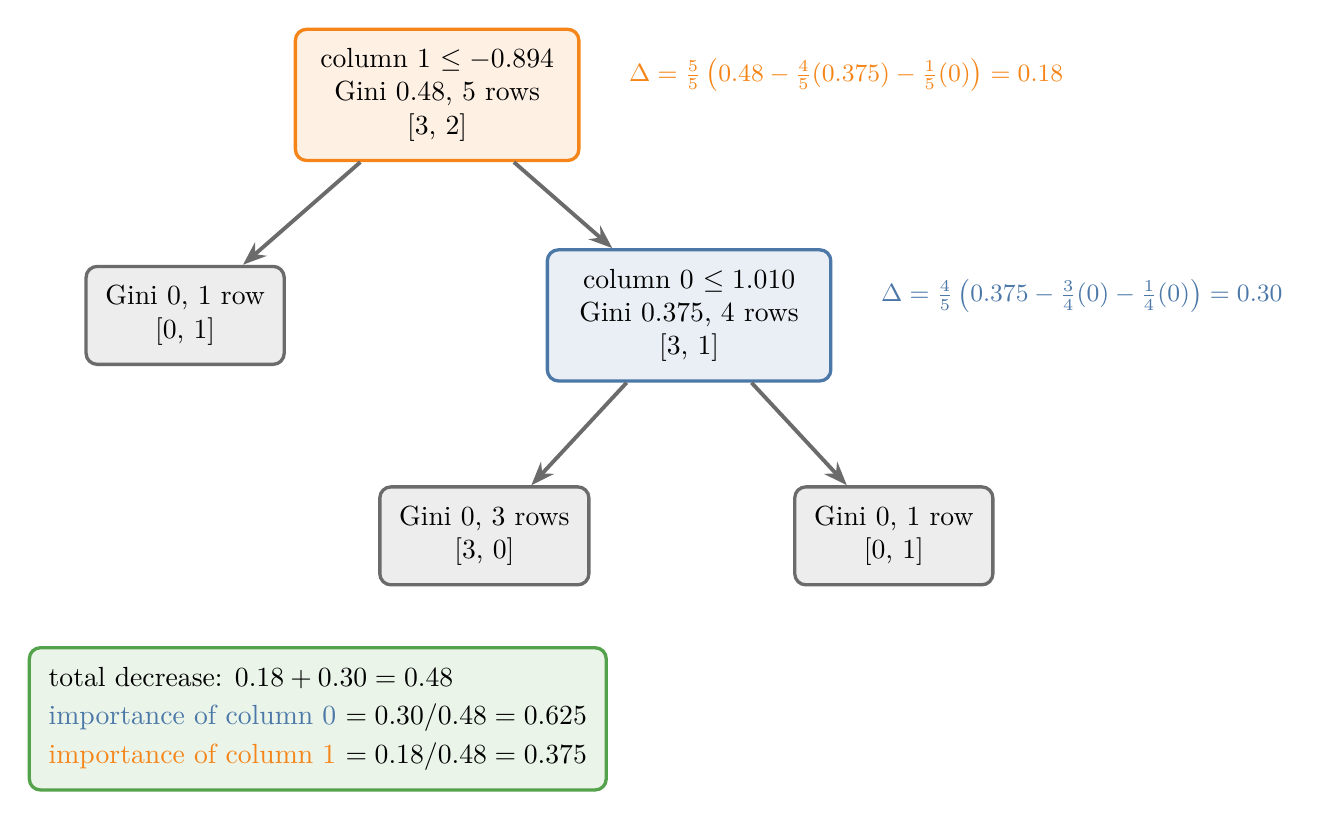
\begin{tikzpicture}[
  s0/.style={box=cblue, minimum width=3.6cm},
  s1/.style={box=corange, minimum width=3.6cm},
  leaf/.style={box=cgrey, minimum width=2.4cm},
  d/.style={font=\sffamily\small, align=left, anchor=west}]
  \node[s1] (r) at (0,0) {column 1 $\le -0.894$\\Gini 0.48, 5 rows\\{[}3, 2{]}};
  \node[leaf] (l1) at (-3.2,-2.8) {Gini 0, 1 row\\{[}0, 1{]}};
  \node[s0] (n2) at (3.2,-2.8) {column 0 $\le 1.010$\\Gini 0.375, 4 rows\\{[}3, 1{]}};
  \node[leaf] (l2) at (0.6,-5.6) {Gini 0, 3 rows\\{[}3, 0{]}};
  \node[leaf] (l3) at (5.8,-5.6) {Gini 0, 1 row\\{[}0, 1{]}};
  \foreach \a/\b in {r/l1, r/n2, n2/l2, n2/l3} \draw[arrow] (\a) -- (\b);
  \node[d, text=corange] at (2.3,0.25) {$\Delta = \frac{5}{5}\left(0.48 - \frac{4}{5}(0.375) - \frac{1}{5}(0)\right) = 0.18$};
  \node[d, text=cblue] at (5.5,-2.55) {$\Delta = \frac{4}{5}\left(0.375 - \frac{3}{4}(0) - \frac{1}{4}(0)\right) = 0.30$};
  \node[box=cgreen, align=left, anchor=north west] at (-5.2,-7.0) {%
    total decrease: $0.18 + 0.30 = 0.48$\\[2pt]
    {\color{cblue}importance of column 0} $= 0.30 / 0.48 = 0.625$\\[2pt]
    {\color{corange}importance of column 1} $= 0.18 / 0.48 = 0.375$};
\end{tikzpicture}
\end{document}
